\documentclass[11pt]{article}

% some definitions for the title page
\newcommand{\reporttitle}{Image Registration}
\newcommand{\reportdescription}{}

% load some definitions and default packages
%---------------------------------------------------------------------------
%	PACKAGES AND OTHER DOCUMENT CONFIGURATIONS
%---------------------------------------------------------------------------

\usepackage[twoside]{fancyhdr}
\usepackage{csquotes}

\usepackage[a4paper,hmargin=2.0cm,vmargin=1.0cm,includeheadfoot]{geometry}
% \usepackage{natbib} % for bibliography
\usepackage{biblatex}
\usepackage{tabularx,longtable,multirow,subfigure,caption}%hangcaption
\usepackage{fancyhdr} % page layout
\usepackage{url} % URLs
\usepackage[english]{babel}
\usepackage{amsmath}
\usepackage{graphicx}
\usepackage{dsfont}
\usepackage{epstopdf} % automatically replace .eps with .pdf in graphics
% \usepackage{backref} % needed for citations
\usepackage{array}
\usepackage{latexsym}
\usepackage[pdftex,hypertexnames=false,colorlinks]{hyperref} % provide links in pdf (had pagebackref)
\usepackage{booktabs}
\usepackage{wrapfig}
\usepackage{caption}  % Required for \captionof
\usepackage{float} % for H option in figures
\usepackage{amssymb}
\usepackage{amsmath}
\usepackage[nottoc]{tocbibind}

%%% Default fonts
\renewcommand*{\rmdefault}{bch}
\renewcommand*{\ttdefault}{cmtt}

%%% Default settings (page layout)
\setlength{\parindent}{0em}  % indentation of paragraph
\setlength{\parskip}{.3em}

\setlength{\headheight}{14.5pt}
\pagestyle{fancy}

\fancyfoot[ER,OL]{\thepage}%Page no. in the left on odd pages and on right on even pages

\fancyfoot[OC,EC]{\sffamily }
\renewcommand{\headrulewidth}{0.1pt}
\renewcommand{\footrulewidth}{0.1pt}
\captionsetup{margin=10pt,font=small,labelfont=bf}
% Here, you can define your own macros. Some examples are given below.

\newcommand{\R}[0]{\mathds{R}} % real numbers
\newcommand{\Z}[0]{\mathds{Z}} % integers
\newcommand{\N}[0]{\mathds{N}} % natural numbers
\newcommand{\C}[0]{\mathds{C}} % complex numbers
\renewcommand{\vec}[1]{{\boldsymbol{{#1}}}} % vector
\newcommand{\mat}[1]{{\boldsymbol{{#1}}}} % matrix

\usepackage{pifont,mdframed}
\newenvironment{warning}
  {\par\begin{mdframed}[linewidth=1pt,linecolor=black]%
    \begin{list}{}{\leftmargin=1cm
                   \labelwidth=\leftmargin}\item[\Large\ding{43}]}
  {\end{list}\end{mdframed}\par}

%\bibliography{bibliography}

\begin{document}

% Include the title page
\begin{titlepage}

    \newcommand{\HRule}{\rule{\linewidth}{0.5mm}} % Defines a new command for the horizontal lines, change thickness here
    
    \center % Center everything on the page
     
    %------------------------------------------------------------------------
    %	HEADING SECTIONS
    %------------------------------------------------------------------------
    
    \textsc{\Large Department of Computing}\\[0.5cm] 
    \textsc{\large Imperial College of Science, Technology and Medicine}\\[0.5cm] 
    
    %------------------------------------------------------------------------
    %	TITLE SECTION
    %------------------------------------------------------------------------
    
    \HRule \\[0.4cm]
    { \huge \bfseries \reporttitle}\\ % Title of your document
    \HRule \\[0.4cm]

    \textit{\reportdescription}
    
    \vspace{2em}

    %------------------------------------------------------------------------
    %	AUTHOR SECTION
    %------------------------------------------------------------------------
    
    \large \emph{Author: Anton Zhitomirsky}

    \vspace{1em}

    \global\let\newpagegood\newpage
    \global\let\newpage\relax
    
\end{titlepage}

\global\let\newpage\newpagegood

\tableofcontents

\clearpage

\section{Inverse Problems in Imaging}

\begin{minipage}[l]{.5\linewidth}
    \begin{figure}[H]
        \centering
        \fbox{\includegraphics[page=4, trim=2cm 2cm 2cm 3cm, clip, width=.95\linewidth]{05 - Inverse Problems.pdf}}
    \end{figure}    
\end{minipage}\hfill
\begin{minipage}[r]{.48\linewidth}
    The matrix $A$ operates on some input $x$ which generates an output with noise $n$. We want to try to reconstruct the original input out of the output. 
    
    For example, \textbf{Inpainting}, matrix $A$ would act as a masking operator.
\end{minipage}

\subsection{Classical Approach}

\subsubsection{Problem}

\begin{minipage}[l]{.5\linewidth}
    \begin{figure}[H]
        \centering
        \fbox{\includegraphics[page=8, trim=2cm 2cm 2cm 3cm, clip, width=.95\linewidth]{05 - Inverse Problems.pdf}}
    \end{figure}    
\end{minipage}\hfill
\begin{minipage}[r]{.48\linewidth}
    \begin{itemize}
        \item In de-blurring, classically we can formulate this as a least squares problem, equation on the left. $A$ descibes the forward map (here a linear operation). In other words, after applying a blurring operation to x we get y. 
        \item The solution to this problem includes matrix manipulation.
        \item You can solve the problem without knowing what $A$ is, but here we do.
    \end{itemize}
\end{minipage}

The problem here, is that if the dat is slightly different, then you apply the same deep blurring approach, by solving the least squares solution at the bottom, you can potentially get wildly different solutions with a slightly different initial condition. This is called a \textbf{ill-posed problem} (where a slight pertubation in the data can skew results greatly).

\subsubsection{Solution}

\begin{minipage}[l]{.5\linewidth}
    \begin{figure}[H]
        \centering
        \fbox{\includegraphics[page=10, trim=2cm 2cm 2cm 3cm, clip, width=.95\linewidth]{05 - Inverse Problems.pdf}}
    \end{figure}    
\end{minipage}\hfill
\begin{minipage}[r]{.48\linewidth}
    Even with classical methods you can solve this by adding a regularisation term.
    \begin{itemize}
        \item In addition to minimising the distance between the observed data and the forward operation on the original data, you add a second term
        \item The second term in this example is a regularisation term, which is added to the solution, which modifies the behaviour of the optimisation problem. 
    \end{itemize}
\end{minipage}

\begin{itemize}
    \item This gives a different solution (we effectively add an identity matrix scaled by lambda before we invert $A^\top A$). The $\lambda$ defines the strength of the regularisation; if you increase $\lambda$ you get smoother solutions because you pay less and less attention to the actual distance measure which you have in the first term.
    \item This inversion means that $A^\top A$ becomes better conditioned, which means it's numerically more stable and you suppress noise.
\end{itemize}

\subsection{General Approach}

\begin{minipage}[l]{.5\linewidth}
    \begin{figure}[H]
        \centering
        \fbox{\includegraphics[page=12, trim=2cm 2cm 2cm 3cm, clip, width=.95\linewidth]{05 - Inverse Problems.pdf}}
    \end{figure}    
\end{minipage}\hfill
\begin{minipage}[r]{.48\linewidth}
    \begin{itemize}
        \item This regluarisation approach encodes the prior knowledge we have on our desired solution $x$.
        \item If we can encode this prior knowledge then we have a good regularisation strategy.
        \item The common regularisers shown to the side don't operate on image intensities, but rather on the image gradient. 
        \item For example, the Tikhonov regularisation uses L-2 norm to regularise the gradients of the image intensities
    \end{itemize}
\end{minipage}
\begin{itemize}
    \item The second term, minimises the L-1 norm of the gradient of image intensities. 
    \item Another common solution is to not regularise the image intensities of the gradient of image gradients, but first apply a sparsifying transformation, e.g. wavelet and then minimise that.
\end{itemize}

\subsubsection{Why normalize gradients instead of image intensities?}

\begin{minipage}[l]{.5\linewidth}
    \begin{figure}[H]
        \centering
        \fbox{\includegraphics[page=13, trim=2cm 2cm 2cm 3cm, clip, width=.95\linewidth]{05 - Inverse Problems.pdf}}
        
    \end{figure}    
\end{minipage}\hfill
\begin{minipage}[r]{.48\linewidth}
    \begin{itemize}
        \item The problem with looking only at the gradients, is that the results are very sparse, which is a common thing in every-day images. 
        \item If you apply L-1 norm on the wavelength decomposition, then you're effectively minimising the number of non-zero wavelength coefficients. This technique uses this wave decomposition in order to maximise sparsity or minimise the L-1.
    \end{itemize}    
\end{minipage}

\begin{itemize}
    \item The third approach is \textbf{Dictionary Learning} where you extract small patches from the iamge and build up a patch library. Then you encode each patch by a sparse combination of (e.g.) wavelet coefficients, denoising and combine these to reconstruct the original image.
\end{itemize}

\subsection{Regularisation in inverse problems}

\begin{minipage}[l]{.5\linewidth}
    \begin{figure}[H]
        \centering
        \fbox{\includegraphics[page=14, trim=2cm 2cm 2cm 3cm, clip, width=.95\linewidth]{05 - Inverse Problems.pdf}}
        
    \end{figure}    
\end{minipage}\hfill
\begin{minipage}[r]{.48\linewidth}
    \begin{itemize}
        \item we have an optimisation function made of two terms, the data consistency term and the regularisation.
        \item Can we learn a reguliser from our data rather than using these very ad hoc measures. 
    \end{itemize}
\end{minipage}

\subsection{Forward model/inverse model}

\begin{figure}[H]
    \centering
    \subfigure[image super resolution, the forward model is easy to implement. The inverse is harder]{
        \fbox{\includegraphics[page=15, trim=3cm 5cm 3cm 6cm, clip, width=.3\linewidth]{05 - Inverse Problems.pdf}}
    }
    \subfigure[image super resolution, the forward model can be implemented here, wheras the reverse is a black box called the super resolution algorithm.]{
        \fbox{\includegraphics[page=16, trim=3cm 5cm 3cm 6cm, clip, width=.3\linewidth]{05 - Inverse Problems.pdf}}
    }
    \subfigure[In-painting, the forward model is sipmle; just mask out image intensities. The inpainting tries to recover these masked values]{
        \fbox{\includegraphics[page=17, trim=3cm 5cm 3cm 6cm, clip, width=.3\linewidth]{05 - Inverse Problems.pdf}}
    }
\end{figure}    

\section{Solving Inverse Problems with Deep Learning}

There are three classes of methods

\begin{enumerate}
    \item Model agnostic (ignores forward model)
    \item Decoupled (First learn, then reconstruct)
    \item Unrolled optimisation
\end{enumerate}

\subsection{Model Agnostic Approach}

\subsubsection{Solving the inverse problems}

\begin{figure}[H]
    \centering
    \subfigure{
        \fbox{\includegraphics[page=20, trim=3cm 3cm 3cm 6cm, clip, width=.45\linewidth]{05 - Inverse Problems.pdf}}
    }
    \subfigure{
        \fbox{\includegraphics[page=21, trim=3cm 3cm 3cm 6cm, clip, width=.45\linewidth]{05 - Inverse Problems.pdf}}
    }
\end{figure}    

Assume that the paired data ($x,y$) which are easy to generate. Then take a neural network to solve the inverse problem. The issue here, is that you don't use any information about what happened in the forward operation. The model can be made more intelligent by being partly model agnostic; we can upsample using a classsical algorithm, like linear interpolation, which aren't perfect but produce something useful. Then, after this approximation, you can train a network to remove the difference between the upsampled version (which may have artifacts) and the original.

\subsection{Decoupled Approach}

\subsubsection{Deep Proximal Gradient}

\begin{minipage}[l]{.5\linewidth}
    \begin{figure}[H]
        \centering
        \fbox{\includegraphics[page=22, trim=1cm 2cm 1cm 3cm, clip, width=.95\linewidth]{05 - Inverse Problems.pdf}}
        
    \end{figure}    
\end{minipage}\hfill
\begin{minipage}[r]{.48\linewidth}
    \begin{itemize}
        \item We're still trying to solve an optimization problem, this time with an iterative optimization. 
        \item Compute one step that minimises $D$ and one step that minimises the image regularsiation term. We estimate using gradient descent. 
        \item The second equation is replaced with a nerual network, which takes the estimate from the gradient descent step and produces a new estimate for the data.
    \end{itemize}
\end{minipage}

\subsubsection{General Adversarial Network}

\begin{minipage}[l]{.5\linewidth}
    \begin{figure}[H]
        \centering
        \fbox{\includegraphics[page=23, trim=1cm 2cm 1cm 3cm, clip, width=.95\linewidth]{05 - Inverse Problems.pdf}}
    \end{figure}    
\end{minipage}\hfill
\begin{minipage}[r]{.48\linewidth}
    \begin{itemize}
        \item We want to learn a regularisation function which gives a value of 0 if the image looks realistic and otherwise an infinitely large value. 
        \item If you're on the image manifold then you generate an image which looks real.
    \end{itemize}
\end{minipage}

\begin{minipage}[l]{.5\linewidth}
    \begin{figure}[H]
        \centering
        \fbox{\includegraphics[page=25, trim=1cm 2cm 1cm 3cm, clip, width=.95\linewidth]{05 - Inverse Problems.pdf}}
    \end{figure}    
\end{minipage}\hfill
\begin{minipage}[r]{.48\linewidth}
    \begin{itemize}
        \item A generator takes a vector of noise and generates images from this noise.
        \item The output is fed into a discriminator along with real images which tries to understand if an image is real or fake.
        \item Both are trained simultaneously 
    \end{itemize}
\end{minipage}

\begin{minipage}[l]{.5\linewidth}
    \begin{figure}[H]
        \centering
        \fbox{\includegraphics[page=27, trim=1cm 2cm 1cm 3cm, clip, width=.95\linewidth]{05 - Inverse Problems.pdf}}
    \end{figure}    
\end{minipage}\hfill
\begin{minipage}[r]{.48\linewidth}
    \begin{itemize}
        \item We can now start plugging in the discriminator or generator into the inverse problem.
        \item We can choose only solutions of $x$ that can be generated from the generator because the generator can only generate realistic looking images. In the optimisation, we can use the generator to generate solutions that look real.
        \item Note here, we have restricted the space to the image mainfold shown above using the generator.
    \end{itemize}
\end{minipage}

Here, we assume that we know $A$.

\subsection{Unrolled optimisation}

\subsubsection{Gradient descent networks}

\begin{minipage}[l]{.5\linewidth}
    \begin{figure}[H]
        \centering
        \fbox{\includegraphics[page=31, trim=1cm 2cm 1cm 3cm, clip, width=.95\linewidth]{05 - Inverse Problems.pdf}}
    \end{figure}    
\end{minipage}\hfill
\begin{minipage}[r]{.48\linewidth}
    \begin{itemize}
        \item if we assume that our regularisation term $\mathcal R$ is differentiable, (which is why we used the proximal gradient algorithm $\arg \min_x \mathcal D(ax,y)+\lambda\mathcal R (x)$)
        \item Then we can minimise the equation, and do a gradient descent step and take a step in the direction of the regularisation.
        \item The first term corresponds to gradient descent for data consistency, and the second for gradient descent for regularisation
    \end{itemize}
\end{minipage}

\begin{itemize}
    \item We can replace the second step with a neural network.
    \item The diagram: shows an iterative optimisation step, where you start with an initial estimate, you add the gradient with respect to data consistency and the gradient with respect to regularisation and make a step in the direction of the combined gradient.
    \item the bottom term was replaced with a nerual network. Originally, it was the $\eta \triangledown \mathcal R [\cdot]$
    \item Since we have pairs of $x,y$ we can simulate the transformation and train the network with the transformed output.
\end{itemize}

\section{Deep Learning for Image Super-Resolution}

\subsection{Problem formulation}

\begin{minipage}[l]{.5\linewidth}
    \begin{figure}[H]
        \centering
        \fbox{\includegraphics[page=33, trim=6cm 8.3cm 6cm 8cm, clip, width=.95\linewidth]{05 - Inverse Problems.pdf}}
    \end{figure}    
\end{minipage}\hfill
\begin{minipage}[r]{.48\linewidth}
    Upsample low-resolution (LR) images to high-resolution (HR or SR) image. The forward model (going from high-to-low-resolution) is straightforward and involves some image degradation followed by downsampling. The Inverse model is for example an interpolation-based model.
\end{minipage}

\subsection{Example Frameworks}

\begin{figure}[H]
    \centering
    \subfigure[We can have a network with a couple of convolutions and some upsampling]{\fbox{\includegraphics[page=34, trim=1cm 2cm 1cm 3cm, clip, width=.45\linewidth]{05 - Inverse Problems.pdf}}}
    \subfigure[Can upsample data to the desired resolution, then have layers to remove artifacts and add details.]{\fbox{\includegraphics[page=35, trim=1cm 2cm 1cm 3cm, clip, width=.45\linewidth]{05 - Inverse Problems.pdf}}}
    \subfigure[A cascade by upsample by increasing factors (by a bit)]{\fbox{\includegraphics[page=36, trim=1cm 2cm 1cm 3cm, clip, width=.45\linewidth]{05 - Inverse Problems.pdf}}}
    \subfigure[upsample then downsample. Compute the error between the two, and use it in future iterations to improve performance.]{\fbox{\includegraphics[page=37, trim=1cm 2cm 1cm 3cm, clip, width=.45\linewidth]{05 - Inverse Problems.pdf}}}
\end{figure}

\subsection{How to implement upsampling?}

\begin{figure}[H]
    \centering
    \fbox{\includegraphics[page=38, trim=1cm 2cm 1cm 5cm, clip, width=.6\linewidth]{05 - Inverse Problems.pdf}}
\end{figure}

\subsection{Loss functions for super-resolution}

\begin{minipage}[l]{.5\linewidth}
    \begin{figure}[H]
        \centering
        \fbox{\includegraphics[page=39, trim=1cm 2cm 1cm 3cm, clip, width=.95\linewidth]{05 - Inverse Problems.pdf}}
    \end{figure}    
\end{minipage}\hfill
\begin{minipage}[r]{.48\linewidth}
    \begin{itemize}
        \item either take the square or absolute difference between intensities depending on the norm chosen.
        \item Or a huber loss function (a mix between L1 and L2)
        \item L1 is not differentiable which causes numerical problems, so people use something that behaves like L1 but is easier to work with. This is the Huber Loss function.
    \end{itemize}
\end{minipage}

\begin{minipage}[l]{.5\linewidth}
    \begin{figure}[H]
        \centering
        \fbox{\includegraphics[page=40, trim=1cm 2cm 1cm 3cm, clip, width=.95\linewidth]{05 - Inverse Problems.pdf}}
    \end{figure}    
\end{minipage}\hfill
\begin{minipage}[r]{.48\linewidth}
    \begin{itemize}
        \item Don't compare L1 and L2 losses between pixel values. Instead, compute activations in a pre-trained network, like a VGG or ResNet, then compute it for the original data and for the upsampled data.
        \item Then compute the loss not in terms of pixel intensities but in terms of activations in the network.
    \end{itemize}
\end{minipage}

\begin{itemize}
    \item The network has been pre-trained on a task to classify objects for instance, then the activations describe the image in more perceptual terms and that might be a better way of computing values. 
\end{itemize}

\begin{figure}[H]
    \centering
    \fbox{\includegraphics[page=41, trim=1cm 2cm 1cm 3cm, clip, width=.6\linewidth]{05 - Inverse Problems.pdf}}
\end{figure}    

\subsection{GANs for Loss}

Recall, that the generator tries to generate realistic looking images, and the discriminator tries to identify which images are real and which ones are fake. You can the generative adversarial networks as a loss function. 

\begin{minipage}[l]{.5\linewidth}
    \begin{figure}[H]
        \centering
        \fbox{\includegraphics[page=44, trim=1cm 2cm 1cm 3cm, clip, width=.9\linewidth]{05 - Inverse Problems.pdf}}
    \end{figure}    
\end{minipage}\hfill
\begin{minipage}[r]{.48\linewidth}
    \begin{itemize}
        \item Generate with a neural network a realistic super-resolved Image
        \item Use the discriminator to identify how realistic the image is looking.
        \item If the discriminator tells me the image is realistic, we have a low cost function, otherwise, we get a high value.
    \end{itemize}
\end{minipage}

\subsection{Deep Image Prior | Parameterizing images via generative networks}

\begin{figure}[H]
    \centering
    \subfigure[Deep image Prior: introduce the idea to repersent an image not by its pixel values, but by the weights of a vector. We take a random fixed vector $z_0$ as input, and optimise the parameters to obtain an iamge $x$ as output.]{\fbox{\includegraphics[page=45, trim=1cm 4cm 1cm 5cm, clip, width=.45\linewidth]{05 - Inverse Problems.pdf}}}
    \subfigure[If you learn the weights in this manner, this works well for natural images.]{\fbox{\includegraphics[page=46, trim=1cm 4cm 1cm 5cm, clip, width=.45\linewidth]{05 - Inverse Problems.pdf}}}    
    \subfigure[Here we see that generating noise is harder, but real images converge quicker. We can use this to solve image-in-painting. We compare the observed image with the parameterisation through the neural network. ]{\fbox{\includegraphics[page=47, trim=1cm 2cm 1cm 3cm, clip, width=.45\linewidth]{05 - Inverse Problems.pdf}}}
\end{figure}      

\subsubsection{Applciation to inpainting}

\begin{figure}[H]
    \centering
    \subfigure{\fbox{\includegraphics[page=48, trim=1cm 3cm 1cm 3.5cm, clip, width=.45\linewidth]{05 - Inverse Problems.pdf}}}
    \subfigure{\fbox{\includegraphics[page=50, trim=1cm 3cm 1cm 3.5cm, clip, width=.45\linewidth]{05 - Inverse Problems.pdf}}}
\end{figure}

Then, the pixels which are masked out by $m$ and optimise the function over all network weights and learn how to do in-painting. We can then reconstruct the iamge by fitting a noise vector into the image, and reconstruct the image. We achive the following by optimising weights and minimising L2 loss between image generated and the observed image minus the occlusions.

\section{Deep Learning for Image Reconstruction}

\begin{figure}[H]
    \centering
    \subfigure{\fbox{\includegraphics[page=53, trim=1cm 2cm 1cm 3cm, clip, width=.45\linewidth]{05 - Inverse Problems.pdf}}}
    \subfigure{\fbox{\includegraphics[page=54, trim=1cm 2cm 1cm 3cm, clip, width=.45\linewidth]{05 - Inverse Problems.pdf}}}
    \caption*{An x-ray scan captures information by measuring the x-ray energy on the opposite side of the emitter as it passes through soft-tissue. This is rotated around the patient}
\end{figure}

\subsection{Going from Sinogram to CT image}

\begin{minipage}[l]{.5\linewidth}
    \begin{figure}[H]
        \centering
        \fbox{\includegraphics[page=55, trim=1cm 2cm 1cm 3cm, clip, width=.95\linewidth]{05 - Inverse Problems.pdf}}
    \end{figure}    
\end{minipage}\hfill
\begin{minipage}[r]{.48\linewidth}
    \begin{itemize}
        \item We know how to solve the forward transform.
        \item However, how do we solve the inverse problem? 
        \item Typically if we have measured a lot of data then you can just compute the inverse radon trasnform but typically you can't do that becuase you dont have enough data. This may be that for example, a patient may have to hold their breath when giving an MR heart scan, so you don't want them in there for long.
    \end{itemize}
\end{minipage}

\begin{figure}[H]
    \centering
    \subfigure[Can also contain artifacts]{\fbox{\includegraphics[page=56, trim=1cm 2cm 1cm 3cm, clip, width=.45\linewidth]{05 - Inverse Problems.pdf}}}
    \subfigure{\fbox{\includegraphics[page=58, trim=1cm 2cm 1cm 3cm, clip, width=.45\linewidth]{05 - Inverse Problems.pdf}}}
\end{figure}    

\subsection{Going from K-space to MR image}

\begin{minipage}[l]{.5\linewidth}
    \begin{figure}[H]
        \centering
        \fbox{\includegraphics[page=59, trim=1cm 2cm 1cm 3cm, clip, width=.95\linewidth]{05 - Inverse Problems.pdf}}
    \end{figure}    
\end{minipage}\hfill
\begin{minipage}[r]{.48\linewidth}
    \begin{itemize}
        \item Similarly, we know the forward problem, but the inverse is harder.
        \item you can't really tell what the original problem was, you can scan something random and the output looks
    \end{itemize}

    The task becomes ``Recover an image $x\in \mathbb K^{N_x}$ from a set of observations $y \in \mathbb K^{N_y}$ which are corrupted by a noise $n\in \mathbb K^{N_y}$, and $A:\mathbb K^{N_x}\rightarrow \mathbb K^{N_y}$ is a linear operator $y=Ax+n$''
\end{minipage}

\begin{minipage}[l]{.5\linewidth}
    \begin{figure}[H]
        \centering
        \fbox{\includegraphics[page=61, trim=1cm 2cm 1cm 3cm, clip, width=.95\linewidth]{05 - Inverse Problems.pdf}}
    \end{figure}    
\end{minipage}\hfill
\begin{minipage}[r]{.48\linewidth}
    \begin{itemize}
        \item We can similarly have an issue with undersampled data.
    \end{itemize}
\end{minipage}

\begin{figure}[H]
    \centering
    \subfigure[How can we formulate the problem? Use as much physics knowledge as possible (we know there is a forier trasnformation), but this gives a noisy intermediate representation. Therefore, use an nn to remove artifacts.]{\fbox{\includegraphics[page=62, trim=1cm 2cm 1cm 3cm, clip, width=.45\linewidth]{05 - Inverse Problems.pdf}}}
    \subfigure[Another approach is to apply an nn to create a new frequency space and then upsample with inverse of forier transform.]{\fbox{\includegraphics[page=63, trim=1cm 2cm 1cm 3cm, clip, width=.45\linewidth]{05 - Inverse Problems.pdf}}}
\end{figure} 

\begin{minipage}[l]{.5\linewidth}
    \begin{figure}[H]
        \centering
        \fbox{\includegraphics[page=68, trim=1cm 2cm 1cm 3cm, clip, width=.95\linewidth]{05 - Inverse Problems.pdf}}
    \end{figure}    
\end{minipage}\hfill
\begin{minipage}[r]{.48\linewidth}
    \begin{itemize}
        \item generate the training data using the forward model
        \item compare the reconstructed image to the ground truth image 
        \item minimise the cost funciton, the losss function between these reconstructed image and ground truth images
        \item back propagation through the neural network in the standard way (e.g. with backpropagation)
    \end{itemize}
\end{minipage}

\begin{figure}[H]
    \centering
    \subfigure[If using the framework above, you need a loss function which is differentiable; so L2 loss between the ground truth image and reconstructed image (MSE) or you can also use the GAN loss funciton]{\fbox{\includegraphics[page=70, trim=1cm 2cm 1cm 3cm, clip, width=.45\linewidth]{05 - Inverse Problems.pdf}}}
    \subfigure[Backpropogation]{\fbox{\includegraphics[page=71, trim=1cm 2cm 1cm 3cm, clip, width=.45\linewidth]{05 - Inverse Problems.pdf}}}
\end{figure} 

\begin{minipage}[l]{.5\linewidth}
    \begin{figure}[H]
        \centering
        \fbox{\includegraphics[page=73, trim=1cm 2cm 1cm 3cm, clip, width=.95\linewidth]{05 - Inverse Problems.pdf}}
    \end{figure}    
\end{minipage}\hfill
\begin{minipage}[r]{.48\linewidth}
    When you do inference, you only need to do a forward pass. Which is different to classical inverse problems because there you need to do that for every new dataset, solve the optimisation problem again.
\end{minipage}

\begin{minipage}[l]{.5\linewidth}
    \begin{figure}[H]
        \centering
        \fbox{\includegraphics[page=75, trim=1cm 2cm 1cm 3cm, clip, width=.95\linewidth]{05 - Inverse Problems.pdf}}
    \end{figure}    
\end{minipage}\hfill
\begin{minipage}[r]{.48\linewidth}
    \begin{itemize}
        \item With less data, reconstruct the image with a forier transform and apply an nn to remove artifacts. 
    \end{itemize}
\end{minipage}

\begin{figure}[H]
    \subfigure[Have an nn which in the image space does de-noising operations]{\fbox{\includegraphics[page=77, trim=1cm 2cm 1cm 3cm, clip, width=.45\linewidth]{05 - Inverse Problems.pdf}}}
    \subfigure[Then also goes with a foreir transform into the signal doimain and makes sure that the data you have reconstructed is consistent with the data you have acquired.]{\fbox{\includegraphics[page=78, trim=1cm 2cm 1cm 3cm, clip, width=.45\linewidth]{05 - Inverse Problems.pdf}}}
\end{figure}

\section{AI-enabled Super resolution Images}

\begin{minipage}[l]{.5\linewidth}
    \begin{figure}[H]
        \centering
        \fbox{\includegraphics[page=83, trim=1cm 2cm 1cm 3cm, clip, width=.95\linewidth]{05 - Inverse Problems.pdf}}
    \end{figure}    
\end{minipage}\hfill
\begin{minipage}[r]{.48\linewidth}
    \begin{itemize}
        \item acquire thick slices through the heart. The data doesn't look very high resolution
    \end{itemize}
\end{minipage}

\begin{figure}[H]
    \centering
    \fbox{\includegraphics[page=84, trim=1cm 2cm 1cm 3cm, clip, width=.95\linewidth]{05 - Inverse Problems.pdf}}
    \caption*{Formula a deep learning pipeline, and take the 3D image and 2d images from which we want to recover our 3D data and devlop a simulation for the forward process and generate pairs of high and low resolution data and train the nn to absorb all the iamges again to a high resolution.}
\end{figure}   

\begin{figure}[H]
    \centering
    \fbox{\includegraphics[page=85, trim=1cm 2cm 1cm 3cm, clip, width=.95\linewidth]{05 - Inverse Problems.pdf}}
    \caption*{This is something you can use a residual network for}
\end{figure}  

% \printbibliography
% \addcontentsline{toc}{section}{Bibliography}

\end{document}